\documentclass[./00PhotoBox.tex]{subfiles}
\graphicspath{{\subfix{./img/}}}
\begin{document}


\chapter{Voruntersuchungen}
\label{c:voruntersuchungen}
Vor und während des Aufbaues des eigentlichen Messsystems wurden einige Voruntersuchungen durchgeführt. Diese dienten dazu, die Machbarkeit des Systems zu prüfen und die notwendigen Schritte zu ermitteln und zu optimieren. Hauptsächlich ging es hierbei um die Ermittlung der Kamerakonstanten und der \Gls{Verzeichnung} der Kamera. Auch die Möglichkeit der Erstellung eines 3D-Modells durch Fokusstacking wurde untersucht. Die einzelnen Untersuchungen werden im Folgenden kurz vorgestellt.

\section{Überprüfung der Kameraauflösung}

\paragraph{These}
Die Angabe der Auflösung in Pixeln täuscht bei günstigen Kameras über die tatsächliche Auflösung hinweg.

\paragraph{Ziel}
Die tatsächliche Auflösung der Kamera soll ermittelt werden. Hierbei spielt neben der reinen Anzahl der Pixel auch die Qualität des Objektives der Kameras eine Rolle.

\paragraph{Vorgehen}
Es wurden Bilder von einem Siemensstern unter verschiedenen Belichtungssituationen und Entfernungen aufgenommen (Beispielaufnahme siehe \autoref{img:siemens}). Anschließend wurde die Größe des Unschärfekreises ermittelt und die Linienauflösung und -größe hieraus nach \cite[S. 161]{luhmann} berechnet. Zum Vergleich wurden die Bilder auch mit einer hochwertigeren Kamera aufgenommen (Spiegelreflexkamera Canon EOS 77D mit EF-S 18-55 mm 1:4-5.6 IS STM).

\begin{align*}
    \text{[Auflösungsvermögen]} & = \frac{\text{[Anzahl Segmente]}}{\pi \cdot \text{[Durchmesser Unschärfekreis]}} \\
    \text{[Liniengröße]}        & = \frac{1}{\text{[Auflösungsvermögen]}}
\end{align*}

\paragraph{Ergebnis}

Der Unschärfekreis war durchschnittlich $28$\,\gls{px} groß (\autoref{img:siemens_beschriftet}). Dies entspricht einer Linienauflösung von 292 Linien pro Millimeter, die Linienbreite beträgt \SI{0,0034}{\milli\metre} beziehungsweise $2,44$\,\gls{px}. Die Linienauflösung ist mit etwa \SI{80}{\percent} der Sensorauflösung sehr hoch. Die Linienbreite in Pixeln entsprach der zum Vergleich genutzten Spiegelreflexkamera. Sie kann im Maximalfall (beste Auflösung) $2$\,\gls{px} betragen, entsprechend je eines weißen und schwarzen Pixels pro Linie.


\begin{figure}
    \centering
    \begin{subfigure}{0.45\textwidth}
        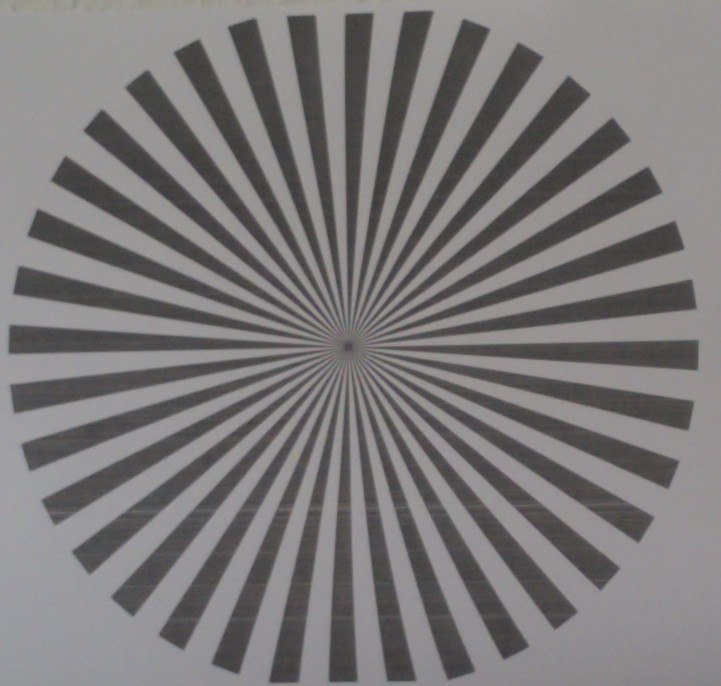
\includegraphics[height=0.9\linewidth]{./img/4_voruntersuchung/siemens.jpg}
        \centering
        \caption{100\%}
        \label{img:siemens}
    \end{subfigure}
    \begin{subfigure}{0.45\textwidth}
        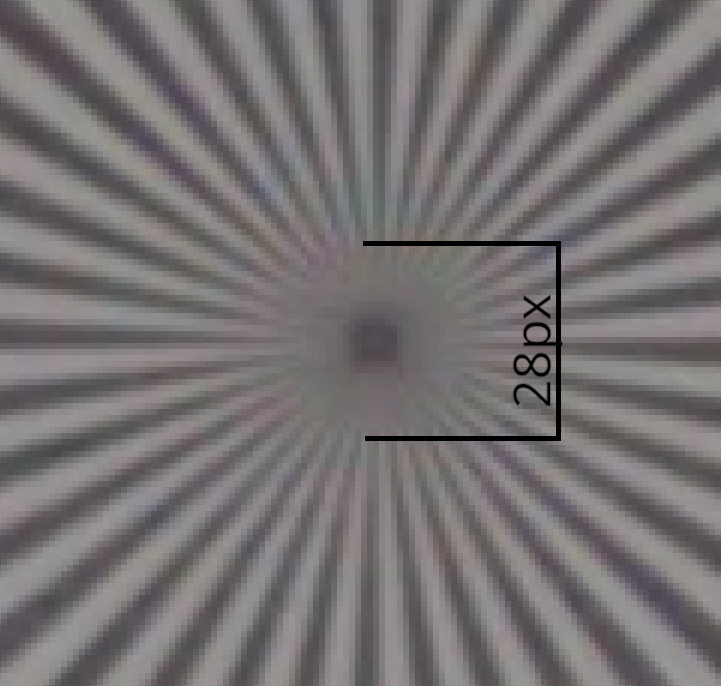
\includegraphics[height=0.9\linewidth]{./img/4_voruntersuchung/siemens_beschriftet.jpg}
        \centering
        \caption{800\%}
        \label{img:siemens_beschriftet}
    \end{subfigure}
    \caption{Siemensstern}
\end{figure}


\section{Änderung der Kamerakonstante durch Fokussierung}
\label{sec:fokus}

\paragraph{These}
Die \Gls{Kamerakonstante} einer Kamera ändert sich durch die Fokussierung. Bei gleich eingestellter Objektdistanz ist die \Gls{Kamerakonstante} näherungsweise gleich.

\paragraph{Ziel}
\citet[S. 59]{kraus} gibt eine Formel (siehe \autoref{eq:kraus_fokus}) für die \Gls{Bildweite} $b$ in Abhängigkeit der Gegenstandsweite $g$ an. Näherungsweise entspricht die \Gls{Bildweite} der \Gls{Kamerakonstante} \citep[S. 59]{kraus}. Die Nutzung der Formel als Näherungswert soll überprüft werden und eine optimierte Formel für die Raspberry-Pi-Kamera ermittelt werden.

\begin{align*}
    \nlabel{eq:kraus_fokus}
    \frac{1}{f} = \frac{1}{g} + \frac{1}{b}
\end{align*}
\begin{conditions}
    f & \Gls{Brennweite} der Kamera \\
    g & Gegenstandsweite \\
    b & Bildweite
\end{conditions}

\paragraph{Vorgehen}
Die Änderungen der Parameter wurden in einem Versuch beobachtet. Hierzu wurde der Raspberry Pi Zero mit montierter Kamera fest vor einem ChArUco-Kalibriermuster platziert. Das Kalibriermuster besteht aus einer Kombination von ArUco-Markern und einem Schachbrettmuster (siehe \autoref{img:charuco}). Durch das Schachbrettmuster ermöglicht es auch bei unscharfen Bildern eine gute automatische Erkennung der zu beobachtenden Punkte. Es wurden je 11 Bilder mit unterschiedlichen Fokussierungen von \SI{2}{\metre} bis  \SI{10}{\centi\metre} aufgenommen. Dieser Vorgang wurde insgesamt viermal wiederholt, um auch die Wiederholungsgenauigkeit zu ermitteln. Die Bilder wurden anschließend mit einem Python-Script unter Nutzung von OpenCV ausgewertet. Hierbei wurde die relative Veränderung der \Gls{Kamerakonstante} ermittelt und mit dem erwarteten Wert verglichen. Die relativen Änderungen wurden auf eine Fokusdistanz von \SI{20}{\centi\metre}, entsprechend einer Fokussierung von \SI{5}{}\,\Gls{dpt}, normiert. Es wurden relative Angaben genutzt, da noch keine genaue Kenntnis über die tatsächliche \Gls{Kamerakonstante} bestand. Die Ergebnisse wurden in einem Box-Whisker-Plot dargestellt.

\begin{figure}
    \centering
    \includegraphics[width=1\textwidth]{./img/4_voruntersuchung/charuco.png}
    \caption{ChArUco-Board mit Fokus auf \SI{5}{}\,\Gls{dpt}}
    \label{img:charuco}
\end{figure}

\paragraph{Ergebnis}
Die Ergebnisse sind in \autoref{img:fokus_faktor} dargestellt. Es zeigt sich, dass die Änderungen der \Gls{Kamerakonstante} durch die Fokussierung linear zu der Dioptrienzahl (Kehrwert der Gegenstandsweite) sind. Ein lineares Verhältnis ergibt sich auch mit der im Datenblatt angegebenen \Gls{Brennweite} von \SI{4,74}{\milli\metre}, jedoch eine etwas flachere Gerade (blau). Die ausgleichende Gerade (rot) ergab eine \Gls{Brennweite} von \SI{6,97}{\milli\metre} (\Gls{Kamerakonstante} bei Fokussierung auf unendlich bzw. \SI{0}{\gls{dpt}}). Die Abweichung von \SI{2,23}{\milli\metre} entspricht einer Abweichung von \SI{47}{\percent}, was als unrealistisch hoch eingeschätzt wird. Hier scheinen sich weitere Effekte bemerkbar zu machen, die noch nicht berücksichtigt wurden. Es wurde daher auch die \Gls{Verzeichnung} weiter untersucht.

\begin{figure}
    \centering
    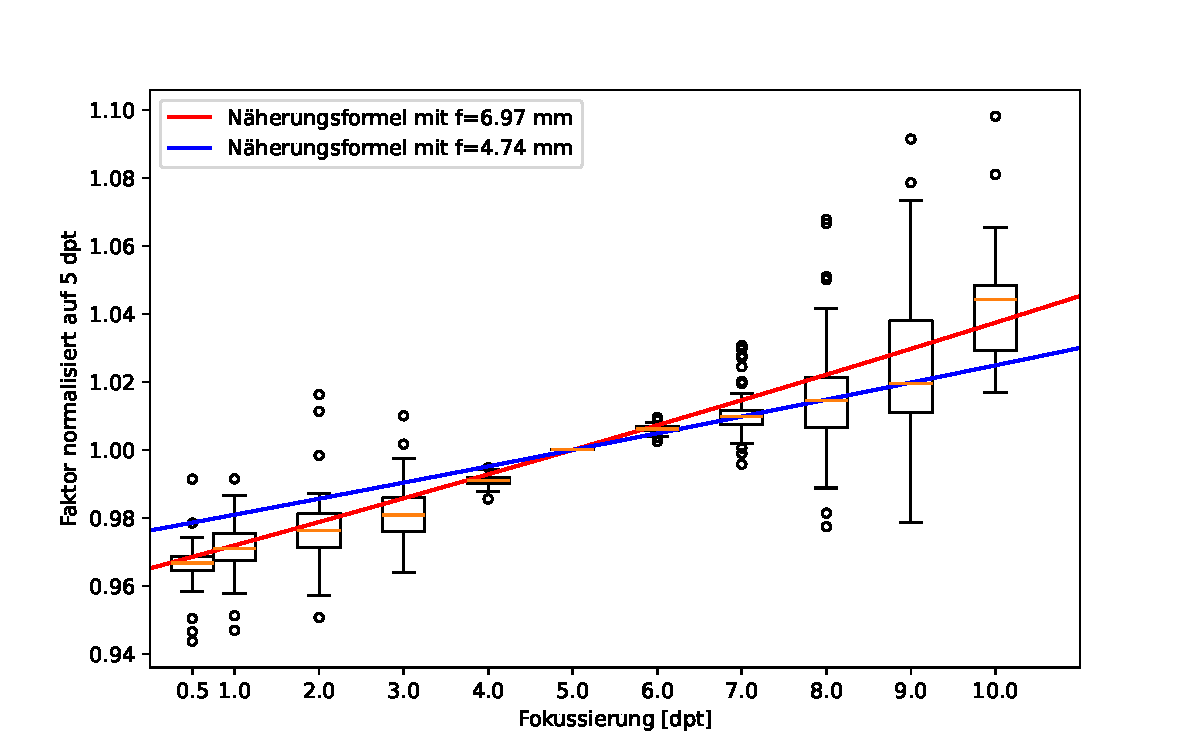
\includegraphics[width=1\textwidth]{./img/4_voruntersuchung/fokus_faktor_diagramm_box.pdf}
    \caption{Box-Whisker-Plot der relativen Veränderung der \Gls{Kamerakonstante} normalisiert auf eine Fokusdistanz von \SI{20}{\centi\metre} (\SI{5}{\glsentryshort{dpt}})}
    \label{img:fokus_faktor}
\end{figure}



\section{Änderung der Verzeichnung durch Fokussierung}

\paragraph{These}
Durch die Verschiebung der Linsen bei der Fokussierung verändert sich auch die \Gls{Verzeichnung} der Kamera.

\paragraph{Ziel}
Die Veränderung der \Gls{Verzeichnung} und eine entsprechende Korrekturformel soll ermittelt werden.

\paragraph{Vorgehen}
Der Versuchsaufbau aus \autoref{sec:fokus} zur Bestimmung der relativen Änderung der \Gls{Kamerakonstante} blieb bestehen. Es wurden jedoch zusätzlich die \Gls{Verzeichnung}en der Bilder ermittelt. Die \Gls{Verzeichnung} wurde mit OpenCV ermittelt und mit der erwarteten \Gls{Verzeichnung} verglichen.

\paragraph{Ergebnis}
Die Ergebnisse waren nicht zufriedenstellend. Es zeigte sich, dass die \Gls{Verzeichnung} mit nur einer Aufnahme pro Fokussierung nicht zufriedenstellend modelliert werden konnte. Es wurde dieses daher erst bei der Kamerakalibrierung weiter untersucht (siehe \autoref{ch:kalibrierung}).


\section{3D-Modell aus Fokusstacking}
\label{sec:fokusstacking}


\paragraph{These}
Die Schärfentiefe der Kameras ist gering. Durch Fokusstacking kann ein besseres 3D-Modell erstellt werden.

\paragraph{Ziel}
Es wird vermutet, dass die geringe Schärfentiefe (siehe \autoref{s:schaerfe}) die Qualität der 3D-Modelle begrenzt. Daher soll geprüft werden, ob durch Fokusstacking die Qualität des 3D-Modell verbessert werden kann.

\paragraph{Vorgehen}
Mittels eines Pythonskriptes wurden die notwendigen Fokusschritte berechnet, damit der Bereich von \SI{10}{\centi\metre} bis \SI{1}{\metre} scharf abgebildet wird. Hierbei wurden die Werte so bestimmt, dass jeweils die hintere Schärfegrenze $a_h$ einer Aufnahme der vorderen $a_v$ des nächsten Bildes entspricht. Im Gegensatz zu den Berechnungen in \autoref{s:schaerfe} wurde hier ein Unschärfekreis von $6$\,\gls{px} akzeptiert, da ansonsten die Anzahl der notwendigen Aufnahmen zu groß geworden wäre. Die berechneten Werte mit ihren Grenzen sind in \autoref{tab:fokusstack} aufgelistet und in \autoref{img:fokusstack_plot} dargestellt -- die blauen Striche stellen hierbei die Abdeckung einer Aufnahme dar.

\begin{table}
    \centering
    \caption{Notwendige Fokusschritte für den Bereich von $0,1$ bis \SI{1}{\metre}} %Tabellenüberschrift
    \label{tab:fokusstack}
    \begin{tabular}{rr|r|r}
        \multicolumn{2}{c|}{\textbf{Fokussierung}} & \multicolumn{1}{c|}{\textbf{Nahgrenze}} & \multicolumn{1}{c}{\textbf{Ferngrenze}}                    \\ \hline
        \multicolumn{1}{r|}{\textbf{{[}m{]}}}      & \textbf{{[}\glsentryshort{dpt}{]}}      & \textbf{{[}m{]}}                        & \textbf{{[}m{]}} \\ \hline
        \multicolumn{1}{r|}{0,11}                  & 9,31                                    & 0,10                                    & 0,12             \\
        \multicolumn{1}{r|}{0,13}                  & 7,93                                    & 0,12                                    & 0,14             \\
        \multicolumn{1}{r|}{0,15}                  & 6,53                                    & 0,14                                    & 0,17             \\
        \multicolumn{1}{r|}{0,19}                  & 5,13                                    & 0,17                                    & 0,23             \\
        \multicolumn{1}{r|}{0,27}                  & 3,72                                    & 0,23                                    & 0,33             \\
        \multicolumn{1}{r|}{0,43}                  & 2,30                                    & 0,33                                    & 0,63             \\
        \multicolumn{1}{r|}{1,15}                  & 0,87                                    & 0,63                                    & 6,66
    \end{tabular}
\end{table}

\begin{figure}
    \centering
    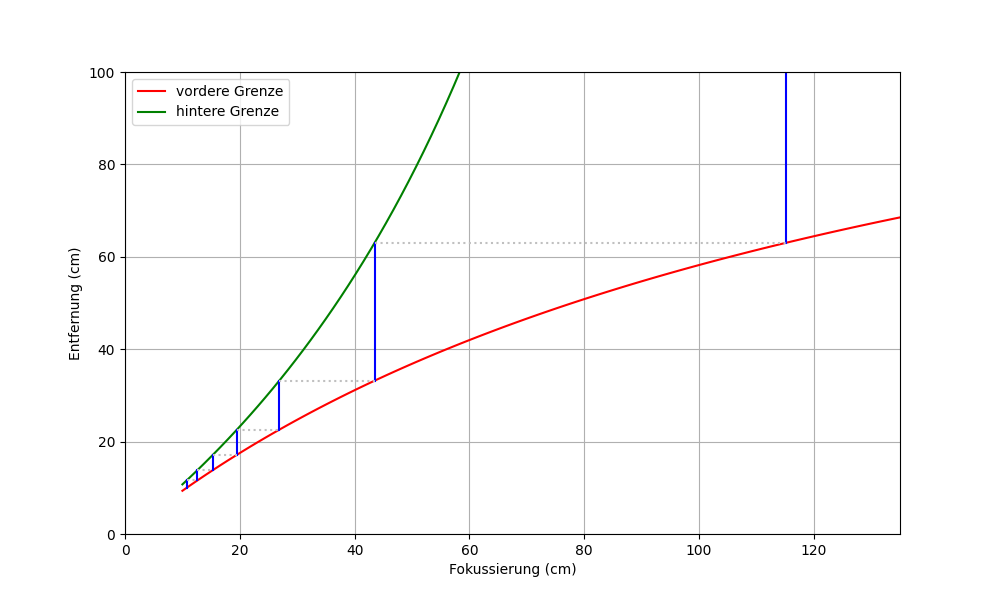
\includegraphics[width=1\textwidth]{./img/4_voruntersuchung/fokusstack_plot.png}
    \caption{Notwendige Fokusschritte, um den Bereich von \SI{10}{\centi\metre} bis \SI{1}{\metre} scharf abzubilden}
    \label{img:fokusstack_plot}
\end{figure}

Anschließend wurden die Bilder mit einem Python-Skript unter Verwendung von OpenCV automatisiert zu je einem Bild pro Kamera bestehend aus allen scharf dargestellten Bereichen zusammengerechnet. Dazu wurde jeweils die notwendige Transformation mittels \Gls{SIFT} (\autoref{ss:sift}) und \Gls{Homografie} berechnet. Die fertigen Bilder wurden dann in Agisoft Metashape zur Berechnung eines 3D-Modells genutzt. Die Daten wurden dann, wie bereits in den vorherigen Untersuchungen beschrieben, mit denen des Streifenprojektionssystems verglichen.

\todo{Bilder von Fokusstacking einfügen}

\paragraph{Ergebnis}
Die Genauigkeit der Passpunkt in Agisoft Metashape bei der Bildverknüpfung ließ zuerst ein erwartetes, besseres Ergebnis vermuten. Jedoch waren die Ergebnisse des 3D-Modelles nicht so wie erhofft, die Qualität des 3D-Modells war schlechter als bei einer einzelnen Aufnahme. Die Flächen des Testy waren kaum mehr vorhanden. Nur mit sehr viel manueller Nacharbeit wurde überhaupt ein erkennbares Ergebnis erzielt. Die Ursache hierfür ist nicht bekannt, aber es wird vermutet, dass die automatische Zusammenrechnung der Bilder zu vielen Artefakten in den Bildern geführt hat, sodass die Bilder dann von der \Gls{SfM}-Software nicht genau genug verknüpft werden konnten. Auch unter Nutzung von kommerziellen Programmen wie Helicon Focus (verwendet von \cite{focusstack_sfm}) und Zerene Stacker waren die Ergebnisse nicht viel besser. Es wurde daher entschieden, den Ansatz erst einmal nicht weiterzuverfolgen.

\section{Überprüfung der Kamerasynchronität}
\label{s:kamerasynchronitaet}
Eine Anforderung war die simultane Auslösung aller Kameras. Um dieses zu überprüfen, wurden die Kameras auf eine Stoppuhr mit Anzeige von Hundertstel Sekunden gerichtet und eine Aufnahme entsprechend der automatischen Aufnahme eines 3D-Modelles durchgeführt. Die Bilder wurden anschließend ausgewertet und hieraus das erste und letzte Bild bestimmt. Dieser Vorgang wurde dreimal wiederholt.

Die Messung zeigte eine Abweichung zwischen dem ersten und letzten Bild von maximal \SI{0,2}{Sekunden}. Die Synchronität der Kameras ist damit für den Anwendungsfall gegeben. Eine Aufnahme von bewegten Objekten ist damit jedoch nicht möglich. Die Abweichung ist auf die unterschiedlichen Reaktionszeiten der Kameras zurückzuführen, auch weil es sich bei dem Betriebssystem der Raspberry Pi nicht um ein Echtzeitbetriebssystem handelt. Außerdem kann die Netzwerkverbindung das Signal weiter verzögern. Die Daten an die verschiedenen Kameras werden zwar gleichzeitig abgesendet, aber durch das Zeitschlitzverfahren des WLAN werden diese nicht gleichzeitig empfangen.
\todo{Zeitschlitz/Echtzeit Quelle}

\biblio
\end{document}